\documentclass{article}
\usepackage{graphicx}
\usepackage{subcaption}

\title{Report 7: Reduction Pattern - Grayscale Stretch}
\author{Nam Le}
\date{\today}

\begin{document}

\maketitle

\section{Method}
I implemented the Grayscale Stretch algorithm based on Slide 47 using a 3-step pipeline:
\begin{enumerate}
    \item \textbf{Step 1 (Map)}: Converted the RGB input image into a 2D grayscale image on GPU using \texttt{rgb\_to\_gray\_gpu}.
    \item \textbf{Step 2 (Reduce)}: Extracted the minimum ($min$) and maximum ($max$) intensity values using Shared Memory parallel reduction kernels (\texttt{reduce\_min\_gpu} and \texttt{reduce\_max\_gpu}) based on Slide 43.
    \item \textbf{Step 3 (Map)}: Recalculated pixel intensity using the stretch formula $g' = \frac{g - min}{max - min} \times 255$ with \texttt{stretch\_gpu}.
\end{enumerate}

\section{Parallel Reduction Logic}
To optimize GPU core usage and eliminate CPU transfer bottlenecks, Step 2 utilizes shared memory caching (\texttt{cuda.shared.array(256, float32)}). Threads perform a binary-tree reduction with stride division ($s = s / 2$) and synchronize via \texttt{cuda.syncthreads()} to prevent race conditions and memory bank conflicts as instructed in Slides 35--43.

\section{Results \& Discussion}
I benchmarked the full execution time across different 2D block size configurations: $(8, 8)$, $(16, 16)$, and $(32, 32)$.

\begin{figure}[h]
    \centering
    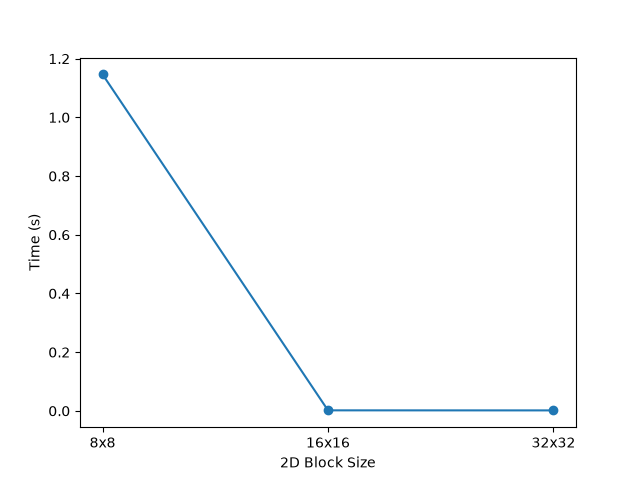
\includegraphics[width=0.7\textwidth]{reduce_block_size_vs_time.png}
    \caption{2D Block Size vs Total Execution Time}
\end{figure}

\begin{figure}[h]
    \centering
    \begin{subfigure}[b]{0.45\textwidth}
        
\includegraphics[width=\textwidth]{input.jpg}
        \caption{Original Image}
    \end{subfigure}
    \hfill
    \begin{subfigure}[b]{0.45\textwidth}
        
\includegraphics[width=\textwidth]{stretched.jpg}
        \caption{Grayscale Stretched Output}
    \end{subfigure}
    \caption{Input vs Output Image for Labwork 7}
\end{figure}

\begin{itemize}
    \item The block configuration $(8, 8)$ took approximately $1.15$ seconds due to low thread occupancy per block.
    \item Configurations $(16, 16)$ and $(32, 32)$ significantly accelerated execution to less than $0.01$ seconds as they fully utilize GPU warps and latency hiding mechanisms.
\end{itemize}

\end{document}

